% doc class visiblement viables : article, scrreprt (écrit plus gros),
\documentclass{article}
\usepackage[francais]{babel}
\usepackage[utf8]{inputenc}  
\usepackage[T1]{fontenc}
\usepackage[colorlinks=true, urlcolor=blue, linkcolor=black]{hyperref} % pour hyper lien
%[colorlinks=true, linkcolor=blue, urlcolor=blue, linktoc=none]
\usepackage{graphicx} % Pour images
\usepackage{listings} % Pour code source
\usepackage{color}    % Pour code source
\usepackage{amssymb} % pour le Checkmark
\definecolor{mygreen}{rgb}{0,0.6,0}
\definecolor{mygray}{rgb}{0.5,0.5,0.5}
\definecolor{mymauve}{rgb}{0.58,0,0.82}
\lstset{ %
  backgroundcolor=\color{white},   % choose the background color; you must add \usepackage{color} or \usepackage{xcolor}
  basicstyle=\footnotesize,        % the size of the fonts that are used for the code
  breakatwhitespace=false,         % sets if automatic breaks should only happen at whitespace
  breaklines=true,                 % sets automatic line breaking
  captionpos=b,                    % sets the caption-position to bottom
  commentstyle=\color{mygreen},    % comment style
  deletekeywords={...},            % if you want to delete keywords from the given language
  escapeinside={\%*}{*)},          % if you want to add LaTeX within your code
  extendedchars=true,              % lets you use non-ASCII characters; for 8-bits encodings only, does not work with UTF-8
  frame=single,                    % adds a frame around the code
  keepspaces=true,                 % keeps spaces in text, useful for keeping indentation of code (possibly needs columns=flexible)
  keywordstyle=\color{blue},       % keyword style
  language=Python,                 % the language of the code
  otherkeywords={*,...},            % if you want to add more keywords to the set
  numbers=left,                    % where to put the line-numbers; possible values are (none, left, right)
  numbersep=5pt,                   % how far the line-numbers are from the code
  numberstyle=\tiny\color{mygray}, % the style that is used for the line-numbers
  rulecolor=\color{black},         % if not set, the frame-color may be changed on line-breaks within not-black text (e.g. comments (green here))
  showspaces=false,                % show spaces everywhere adding particular underscores; it overrides 'showstringspaces'
  showstringspaces=false,          % underline spaces within strings only
  showtabs=false,                  % show tabs within strings adding particular underscores
  stepnumber=1,                    % the step between two line-numbers. If it's 1, each line will be numbered.5
  stringstyle=\color{mymauve},     % string literal style
  tabsize=2,                       % sets default tabsize to 2 spaces
  title=\lstname                   % show the filename of files included with \lstinputlisting; also try caption instead of title
}
%\newcommand{code}[2]{
%hrulefill
%subsection*{#1}
%lstinputlisting{#2}
%vspace{2em}
%}.5
%\usepackage{python}
 
\begin{document}

  \title{Rapport: Arkanoid}
  \author{MASSAVIOL Mathieu\and BRESSAND Jérémy \and BARRY Amadou Bailo \and JULIEN Marin}

  
%http://en.wikibooks.org/wiki/LaTeX/Title_Creation
\begin{titlepage}
  \begin{center}
    
\includegraphics[width=0.25\textwidth]{img/um.png}\\[2em]
    \textsc{\LARGE Université de Montpellier}\\[1em]
    \textsc{\Large Projet de L2 info}\\[5em]
    
    \rule[0.5ex]{\textwidth}{0.1mm}
    \textsc{\Huge \bfseries Arkanoid}\\
   \rule[0.5ex]{\textwidth}{0.1mm}
  \end{center}

  \noindent
  \begin{minipage}[t]{0.5\textwidth}
    \begin{flushleft} \large
    \emph{Auteurs:}\\
    \textsc{BRESSAND} Jérémy\\
    \textsc{MASSAVIOL} Mathieu\\
    \textsc{BARRY} Amadou Bailo\\
    \textsc{JULIEN} Marin\\
    \end{flushleft}
  \end{minipage}%
  \begin{minipage}[t]{0.5\textwidth}
    \begin{flushright} \large
      \emph{Encadrant:} \\
      Mickael \textsc{MONTASSIER}
      \end{flushright}
    \end{minipage}
  \vspace*{\fill}
  \begin{center}
    {\large \today}
  \end{center}
\end{titlepage}


  \tableofcontents
  \newpage
  \section{Problématique}

Le sujet de notre Projet informatique de L2 est la production d'un jeu de type casse brique, à  l'image d'\href{http://fr.wikipedia.org/wiki/Arkanoid}{Arkanoid}.
Son but pédagogique est de fournir un programme à étudier à des étudiants en parcours Physique.
La plupart des logiciels utilisés par les physiciens sont codés en Python. Une demande du client est d'utiliser ce langage pour notre projet.
Aussi il nous a été demandé d'utiliser la bibliothèque tkinter, permettant une gestion simple d'éléments graphiques. Dans un souci de simplicité, on a choisi de manipuler des rectangles. 
Le type de jeu de notre projet nous permet d'aborder de façon pédagogique un ensemble de concept de programmation, tels que
les structures de contrôles, les strucures de données, la manipulation des types de base python (liste, tuple, dictionnaire) et des fichiers ainsi que la gestion des exceptions.
Conformément à la demande du client, nous rendrons notre projet sous deux formes différentes, impérative et orientée objet.
                                   
Arkanoid est un jeu d'arcade conçu par Akira Fujita, développé et édité par Taito. Ce jeu sorti en 1986 sur borne d'arcade est un casse brique. C'est un jeu de dextérité où l'on contrôle un vaisseau spatial en forme de barre. Ce jeu possède une histoire simple : après la destruction par une attaque extraterrestre du vaisseau Arkanoid, un vaisseau rescapé nommé Vaus est envoyé dans une autre dimension pour se venger et détruire Doh l'alien responsable de l'attaque. 
Le jeu se compose d'une balle, d'une barre et de briques. Le but est de casser les briques grâce à la balle que l'on fait rebondir. Le joueur perd lorsqu'il perd la balle.

    \title{Cahier des charges}
  \author{MASSAVIOL Mathieu, BRESSAND Jérémy, BARRY Amadou Bailo, JULIEN Marin}
  \section{Cahier des charges}
  \subsection{Fonctionnalités attendues}
  
  
  Le jeu dispose d'un écran d'accueil et de fin et est doté d'un système de score persistant.
  
  Les éléments de jeu sont les briques, la barre, les murs, les balles et les bonus.
  Une balle rebondit sur les murs, la barre et les briques. On peut disposer de plusieurs balles.
  Lors de la collision balle/barre, la balle est dirigée du côté touché de la barre.
  La barre est contrôlée par le joueur via souris ou clavier.
  % (Lors du rebond de la balle sur la barre, l'angle entre la trajectoire de la balle et l'axe des abscisses est calculé proportionellement à la distance du point d'impact de la balle par rapport à l'extrémité droite de la raquette. Si la balle tape sur l'extrémité droite alors son angle sera minimal. Sinon si la balle tape sur l'extrémité gauche alors son angle sera maximal. Sinon son angle sera compris entre l'angle minimal et maximal en fonction de la distance entre le point d'impact et l'extrémité droite de la barre. )
  Le jeu sera dôté des modes :
  \begin{description}
    \item[Campagne] sa suite de niveaux est écrite à l'avance;
    \item[Arcade] sa suite de niveaux est générée procéduralement à partir d'une graine;
    \item[Coop] deux joueurs jouent avec deux barres en coopération.
  \end{description}
  Lorsque le joueur ne rattrape pas la dernière balle avec la barre, il perd une vie. Lorsqu'il a perdu toutes ses vies, la partie est finie.
  Alors, si le score du joueur entre dans le top10, il y est inscrit. Le top10 est alors réorganisé.

  \subsubsection{Brique}
  Les briques peuvent encaisser un nombre déterminé de coups qui leur est propre. Passé ce nombre, elles sont détruites.
  Elles peuvent avoir un type special, leur attribuant un comportement propre.
  On aura notamment les briques explosives : lors de leurs destructions, elles endommagent les briques environnantes.
  Lorsque que toutes les briques destructibles sont détruites, le niveau est fini. On passe alors à un autre niveau.
  Lorsqu'une brique est détruite, un nombre de points est ajouté au score du joueur. Un bonus peut alors aussi être lâché.

  \subsubsection{Bonus}
  Un bonus descend progressivement. S'ils entrent en collision avec la barre, ils deviennent effectifs.
  Ils déclenchent les effets suivant :
  \begin{itemize}
    \item Ajout d'une balle;
    \item Balle de feu;
    \item Agrandissement temporaire de la barre;
    \item Retrecissement temporaire de la barre.
  \end{itemize}

  \subsubsection{Balle}
  Une balle peut temporairement avoir un type special, lui attribuant un comportement propre.
  On aura notamment la balle de feu qui transperce les briques destructibles sur son passage.
  Une balle va de plus en plus vite au cours d'une même vie.

  \newpage
  \subsection{Fonctionnalités supplémentaires}

  \begin{enumerate}
    \item Le joueur peut créer ses propres niveaux grâce à un éditeur de niveau. 
    \item Le programme gère le plein écran.
    \item Gestion de la redimension de la fenêtre.
    \item La barre peut être controlée par une manette.
    \item Si le joueur termine le niveau rapidement, un niveau bonus apparaît lui permettant un gain de points.
    \item Le jeu est doté d'un mode Battle : Deux joueurs partagent une même série de niveaux. Chacun a son aire de jeu, et le premier qui finit la suite de niveau remporte le match.
    \item Certaines briques peuvent tirer. Lorsque la barre est touchée, elle est temporairement immobilisée.
On aura les bonus supplémentaires :
    \begin{enumerate}
      \item Barre gluante : La barre peut temporairement retenir une balle lors d'une collision;
      \item Module laser : La barre peut temporairement tirer des lasers endommageant les briques;
      \item Division des balles en trois petites de tailles inférieures et de vitesses supérieures.
    \end{enumerate}
    \item Le jeu gère des couples de portails, permettant la téléportation de balles.
    \item Lors de collision barre/mur, les éléments de jeu tremblent à la façon d'un tilt de flipper, permettant à la balle de toucher des briques qu'elle ne toucherait pas sinon.
  \end{enumerate}
  \section{Gestion du projet}
  Nous avons décidé d'utiliser Python3 pour notre projet. Cela nous a occasioné des problèmes de compatibilité, de nombreux modules étant prévus pour Python2. Nous verrons ici la liste des outils abordés, notre organisation et les problèmes d'ordre humain rencontrés dans le déroulement du projet.
  
\subsection{Listes des outils abordés}
  \begin{enumerate}
  %\renewcommand{\labelitemi}{$\bullet$}
     \item[\bf Tkinter] Bibliothèque graphique du langage python, permettant la création d'interfaces graphiques et de différentes sortes de widgets.
    \item[\bf Pygame] Bibliothèque graphique de python plus riche que tkinter. N'apportant rien de crucial et s'étant déjà familiarisé avec tkinter, nous ne l'avons pas utilisé.
    \item[\bf Pymunk] Trop complexe : Outil de gestion de contraintes et collisions pour python. Sa complexité et nos délais impartis nous ont empeché de pouvoir l'utiliser.
    \item[\bf PIL] Bibliothèque de chargement d'image. Obsolète.
    \item[\bf Pillow] Fork de PIL non obsolète. Nous n'avons pas réussi à l'utiliser.
    \item[\bf Pickle] Bibliothèque python permettant de transformer un objet python en code binaire et vice versa. Elle est utilisée dans la gestion des scores et des niveaux.
    
    \item[\bf Git] Outil de gestion de version de fichiers. Nous avons notamment eu recours aux :
	\begin{description}
      \item[Branchs] Nous avons utilisés une branche de développement, et une branche contenant les build stables de notre projet. Une capture d'écran de notre working tree est jointe en annexe.
      \item[Wiki] Nous avons utilisé le wiki interne au git pour partager l'ensemble des informations relatives au projet : dates des réunions, comptes rendus, choses à faire dans la semaine, idées, ...
      \item[Issues] Nous les avons utilisés pour rendre compte des bugs à corriger, des features et éventuelles améliorations à ajouter. Une capture d'écran de nos issues est jointe en annexe.
    \end{description}
    \item[\bf Jabber, Skype]  Jabber est un protocole de communication. Suite à des difficultés relatives à son utilisation pour faire des conférences, nous avons utilisé skype.
    \item[\bf Geogebra] Outil de modélisation géométrique. Il nous a permis de modéliser aisément les fonctions associés au vecteur vitesse de la balle après rebond sur la barre.
    \item[\bf Framapad] Service d'édition de texte collaborative en ligne.
    \item[\bf Ganttproject] Logiciel d'édition de diagramme de Gantt.
    \item[\bf LaTeX]
  \end{enumerate}
\subsection{Organisation du travail} % Gantt
	Le travail a été divisé en trois axes majeurs : analyse, conception de notre programme et implémentation.
	
	La première phase s'est notamment composée de réunions pour aligner notre vision du projet. Nous avons d'abord fait de nombreuses suggestions, nous avons débattu à leurs sujets et à terme nous avons posé le cahier des charges avec notre encadrant. Au fur et à mesure de l'apprentissage des outils liés au projet, nous avons allégé notre cahier des charges dans un soucis de réalisme.
	La phase de conception a également necessité plusieurs réunions pour se mettre d'accord sur la structure du projet. L'élaboration de nos algorithmes s'est fait parallèlement à leur implémentation.
	La troisième phase s'est composée du developpement de la version objet suivie de l'impérative.
	
	Un diagramme de Gantt et la liste des {\em work packages} associés sont joints en annexe.
	
    
\subsection{Gestion des ressources humaines}
	Ce projet ayant été une première expérience de travail collaboratif, des tensions sont apparues. Elles ont été liées à des niveaux d'implication différents ou à des divergences de point de vues. Aussi les tâches ont été distribuées au sein du groupe sur la base du volontariat.
	
	Les niveaux d'implication différents des membres du groupe ont été la source d'un gros retard de la version impérative sur la version objet. 

	On a observé un autre désaccord relatif au mode campagne, deux membres du groupe ne s'étant pas compris sur sa définition. D'autres désaccords de moindre ampleur ont également ponctué notre travail.
  \section{Développement technique}
  Nous avons développé notre code de manière modulaire dans l'idée de maximiser notre productivité, et de permettre une manipulation des fichiers et une gestion des bugs plus simple. L'ensemble des variables globales sont contenues dans le fichier {\bf \em config.py}. On notera l'absence de constante en python.
    
  \subsection{Animations}
  Pour concevoir nos animations, l'idée retenue a été de décomposer une animation en deux parties : la classe Animation et la classe ElemAnim.
	

	Un objet Animation contient plusieurs instances d'ElemAnim et ne manipule pas de surfaces dans le canvas. Son rôle est de créer, déplacer et enlever des objets de type ElemAnim. Elle gère ainsi la structure d'une animation, non son apparence.

    Un objet ElemAnim contient des surfaces. Son rôle est d'ajouter, de déplacer, d'enlever et de modifier les propriétés des surfaces du Canvas. ElemAnim gère ainsi l'apparence d'une animation.

    Cette décomposition entre structure et apparence permet de simplifier le code et de le rendre plus lisible.

    Lors de la conception des animations, de nombreuses classes filles de la classe Animation ont été créées ainsi que pour la classe ElemAnim. Il était alors possible de combiner telle classe héritant de Animation avec telle classe héritant de ElemAnim ce qui donnait de la généricité dans notre code.
    Peu satisfaits de l'apparence de ces animations, nous n'avons gardé que peu de ces classes pour le programme final.
	
  \subsection{Collision}
	
  Notre algorithme de collision teste deux entités (balle, brique, ...) et renvoie une liste de dictionnaires que l'on appelle {\em \bf flag}, qui correspond aux modifications à faire ne pouvant être faites en interne du fait de la limite de la portée des variables. Un exemple est la création d'une animation de destruction de brique, le {\em flag} correspondant contient alors le nom et la position de l'événement.

  La stratégie adoptée pour l'algorithme est la suivante :
  \begin{itemize}
    \item En fonction de leurs directions, on teste si les deux entités testées se chevauchent à la prochaine frame -- ie s'il va y avoir collision ;
    \item Si oui, on détermine le type de collision : sur les bord verticaux ou horizontaux ;
    \item On gère toutes les données de collision que la portée des variables nous permet de modifier (direction de la balle après rebond, points de vie des briques, destruction du bonus lors de son ramassage, ...) ;
    \item On retourne les {\em flags} correspondant aux événements n'ayant pu être gérés en interne.
  \end{itemize} 

  \subsection{Génération procédurale}
	La génération procédurale consiste en la génération de contenu de manière algorithmique, par opposition à la lecture de contenu pré-écrit. Nous utilisons ce concept dans nos modes Arcade et Coop pour générer les niveaux à partir d'une graine saisie par l'utilisateur. Une donnée supplémentaire vient compléter la génération : la difficulté. À chaque fois qu'un joueur avance de niveau, elle augmente, assignant aux malus et types de briques désavantageux des probabilités d'apparition supérieures.


    Notre stratégie de génération de niveau est la suivante :
	\begin{itemize}
    \item Génération de bruit blanc plafonné entre 1 et 3, correspondant aux points de vie des briques ;
    \item Suppression de briques, donnant à la disposition des briques une forme autre qu'un grand rectangle ;
    \item La distribution des types spéciaux de briques, limités aux types explosif et indestructible dans la version rendue ;
    \item La distribution des bonus et malus dans les briques ;
    \item Nous retournons finalement notre liste de briques pour permettre son exploitation.
	\end{itemize}
    La fonction principale de notre génération procédurale est disponible en annexe.
  \subsection{Éditeur de niveaux}
  
      Parmi les fonctionnalités supplémentaires de notre cahier des charges nous avons implémenté un éditeur de niveaux qui nous a permis d'écrire facilement les niveaux de notre mode campagne.

    L'éditeur se lance à partir d'un fichier annexe contenant la classe {\bf \em EditeurLvl}. Cette classe comprend comme attributs des variables correspondant aux différents paramètres du constructeur d'une brique ainsi qu'une liste de briques ainsi qu'un compteur incrémenté à chaque ajout de brique. En effet nous avons paramétré plusieurs touches pour pouvoir changer les attributs correspondant à la brique. Une dernière touche (la touche {\em Entrée}) permet de rajouter à la liste de briques une brique avec comme paramètre l'état actuel des attributs de la classe. Lorsque le niveau est rempli (quand le compteur de briques correspond à la taille d'un niveau définie dans {\bf \em config.py}), on appelle la methode de sauvegarde du niveau. Elle crée un nouveau fichier binaire et dans lequel on écrit grâce à la fonction {\em dump} de la bibliothèque {\bf \em pickle} qui prend la liste de briques et la transforme en code binaire.

    Nous  n'avons pas eu le temps de créer un mode de jeu pour jouer au niveaux édités. L'utilisateur peut quand même réécrire la campagne à son gout en  créant des niveaux ayant pour nom 0, 1, ... , 9 qui remplaceront les  fichiers actuels.

  \section{Tests unitaires}
  On introduira ici seulement les tests unitaires nécissant une présentation de leur fonctionnement. On notera aussi que seule la version objet, plus aboutie, en est dotée. On conseillera de les lancer à partir d'un terminal, diverses informations étant censées y être affichés.

  \subsection{Collision}
    Le test unitaire du fichier {\em \bf collision.py} permet de tester les différents types de collisions. Les contrôles sont les suivants :
    \begin{itemize}
    \item clic gauche et mouvement pour déplacer la balle (lui donner une vitesse et direction)
    \item flèches directionnelles pour déplacer la barre
	\end{itemize}
	On trouve en sortie dans le terminal les éléments en collision, le type de collision détecté (vertical, horizontal) et les éventuels {\em flags} non traités à l'intérieur de la fonction de collision. Ils peuvent par exemple correspondre à la création d'un bonus ou d'une animation.

  \subsection{Génération procédurale}
	Le fichier {\em \bf procgen.py} s'éxécute avec un argument correspondant à la graine. À défaut, la graine est définie à 1337. Les petits rectangles verts correspondent à la présence d'un bonus dans une brique, les rouges à des malus. La version fournie étant réglée par défaut à une difficulté de 0\%, aucun malus n'est censé apparaître.
  \section{Conclusion}
  
  \subsection{Autocritique }
    Ce projet ayant été le premier de cette envergure pour nous, nous avons fait diverses erreurs même si nous restons globalement satisfait du produit final.

    Tout d'abord, notre mauvaise gestion du temps et du planning a été à la source de différents problèmes.
    Une de nos erreurs a été de commencer à coder avant d'avoir finaliser tous nos algorithmes. Cela a mener à la production de programme contenant de nombreux bugs -- on pense aux animations et plus encore aux collisions -- et à terme à un code peu intuitif une fois ces bugs résolus.
    La version impérative a souffert d'un retard du même fait de la gestion du temps. Nous avions initialement prévu de les développer en même temps, mais étant donné l'évidente similarité des algorithmes nous avons préféré d'abord produire la version objet et l'adapter en impératif. Aussi des tensions internes ont géné à la production de celle-ci.

    Même si globalement satisfaits de notre projet, force est de constater que des améliorations importantes peuvent être faites. Par exemple, les bonus sont présentement gérés type par type. Il faudrait disposer d'un système permettant d'assigner dynamiquement tel effet sur un élément de jeu à tel bonus; cela permettrait d'ajouter une grande quantité de bonus de manière simple. Une autre amélioration possible aurait été d'assigner de manière automatique un type d'animation à la destruction d'une brique. On aurait par ces deux améliorations largement réduit notre usage des flags lié à la collision, qui sont assez peu pratiques.

    Enfin notre organisation a également souffert de divers problèmes. La répartition des tâches s'étant faite sur la base du volontariat, la charge de travail par membre a été déséquilibré. Une meilleure solution aurait été de se répartir les tâches équitablement.
     Nous avons programmé de manière modulaire, chose qui facilite la compréhension et la réutilisation du code. Aussi nous avons eu des problèmes d'interfaçage, bien que mineurs. Cependant, nous nous sommes trop centrés sur nos tâches respectives. Nous aurions gagné en efficacité en travaillant parallèlement dans la même salle, du fait de la stimulation et de l'échange d'idée qui en serait sorti.
    
  \subsection{Perspective }
    Notre programme connait différentes perspectives d'évolution, principalement grâce à la programmation modulaire et la présence des variables globales dans le fichier config.py.

    Certains fichiers, du fait des ajouts successifs auxquels ils ont été sujet, ont des perspectives d'évolution limité en l'état. C'est notamment le cas pour le module de collision et de gestion des différents modes de jeux.

		Malgré tout, on peut adapter la dimension du jeu par une simple modification des variables globales, comme l'on peut modifier la vitesse des balles, des bonus et barres, la durée des bonus, l'interval de point de vie des briques, ...
    L'utilisation des modules pré-éxistants permettent l'ajout de nouvelles fonctionnalités. Par exemple, l'ajout de l'éditeur de niveau a été postérieur aux autres modules et n'a pas demandé d'adaptation.
  
  \section{Annexe}
  \subsection{Bibliographie}
    \begin{itemize}
    	\item "Apprendre à programmer avec Python 3" - Gérard Swinnen
    	\item \href{http://effbot.org/}{http://effbot.org/}
    \end{itemize}

  \subsection{Liste des Work Packages}
  \begin{figure}[h!]
    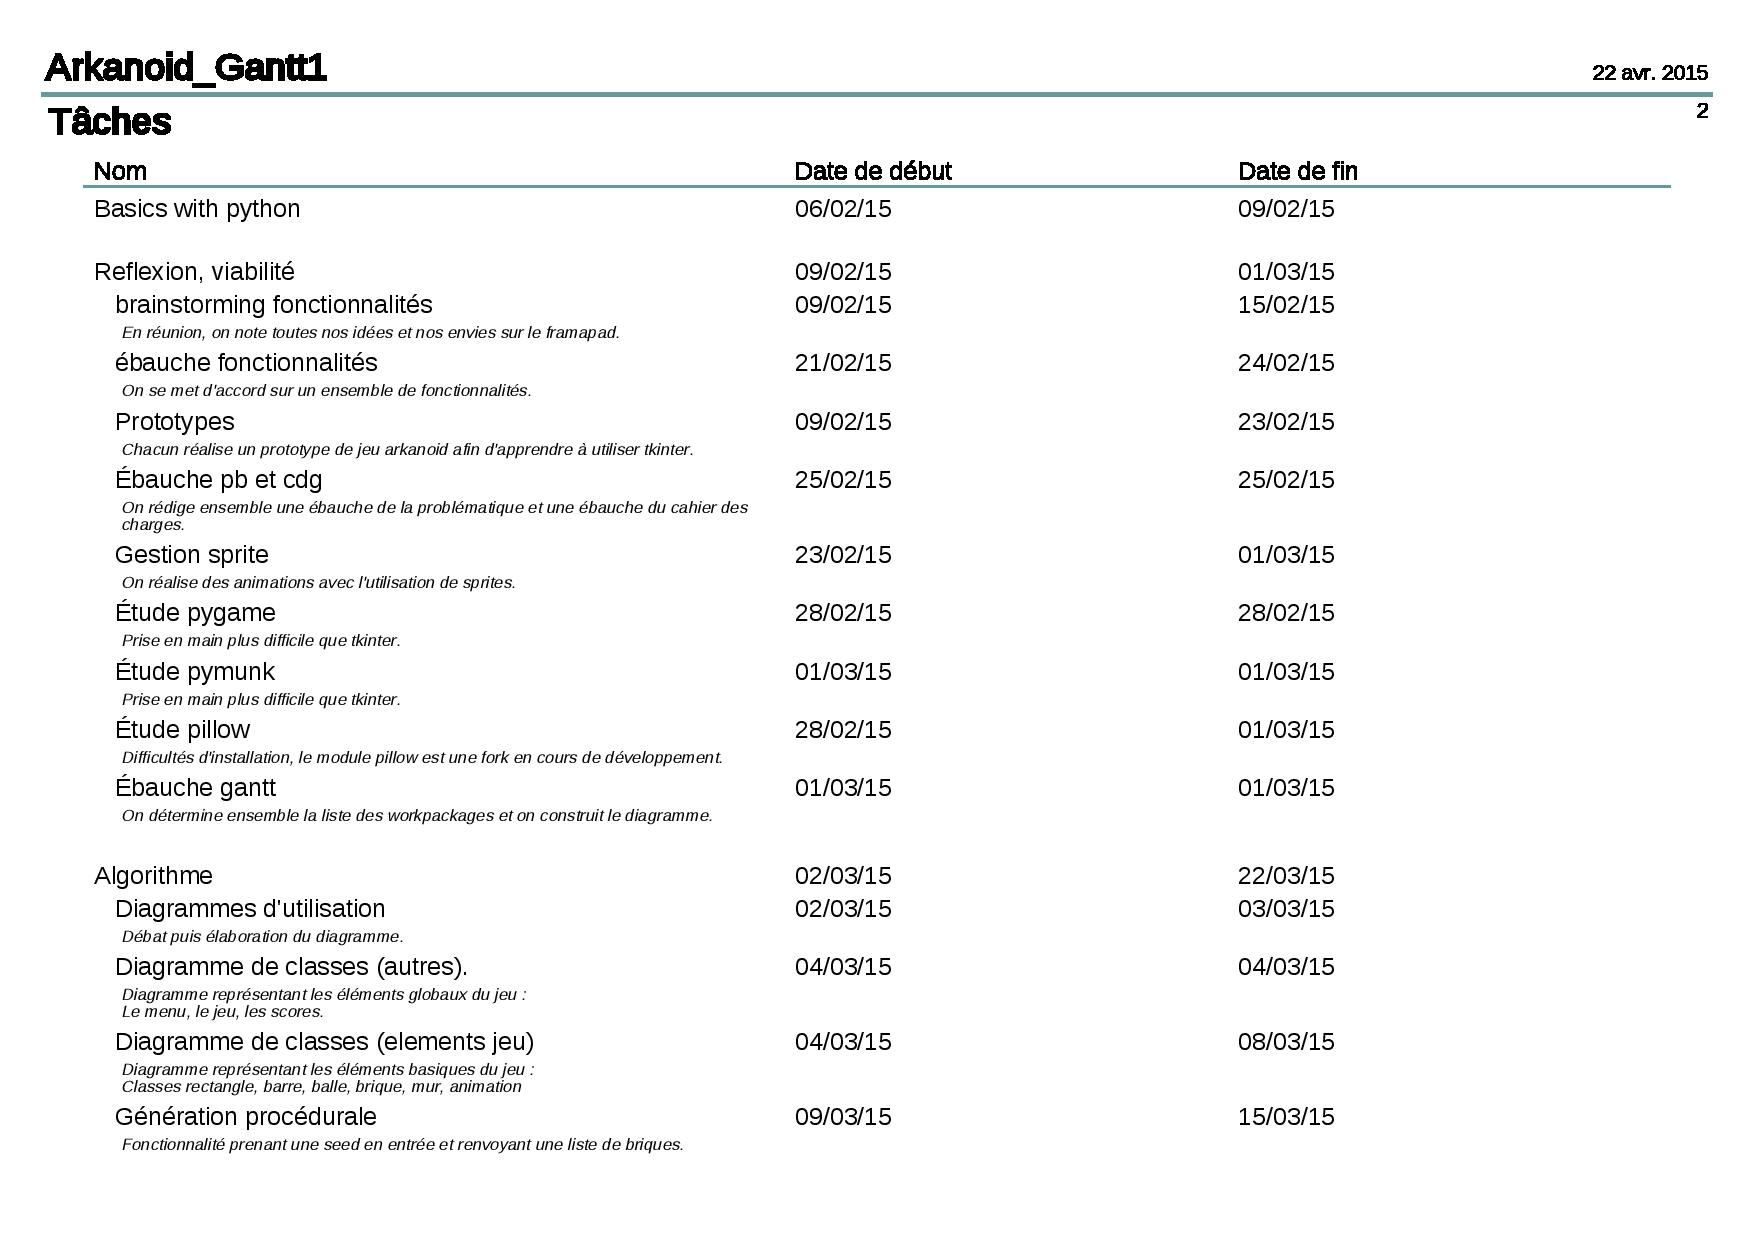
\includegraphics[width=1\textwidth]{img/WK1.jpg}\\
  \end{figure}
  \begin{figure}[h!]
    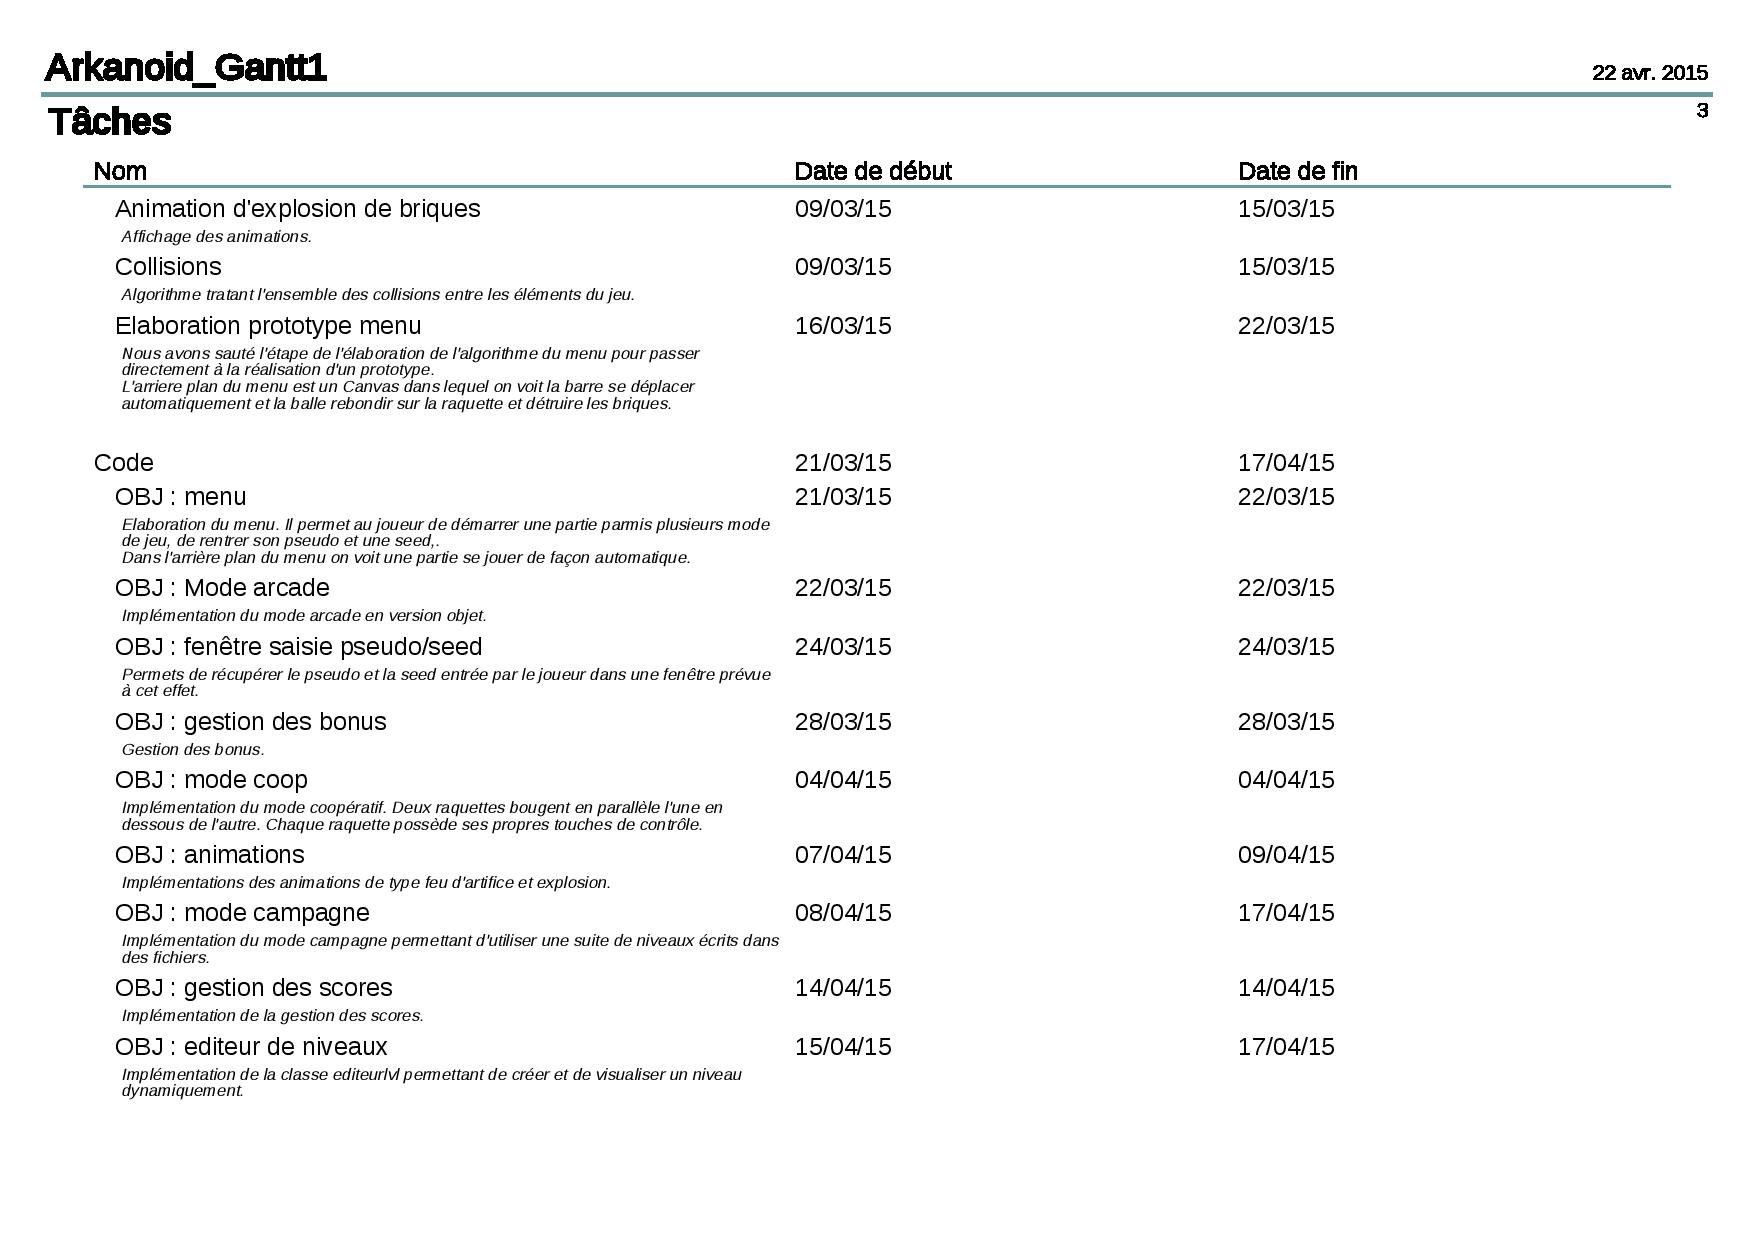
\includegraphics[width=1\textwidth]{img/WK2.jpg}\\
  \end{figure}
  \begin{figure}[h!]
    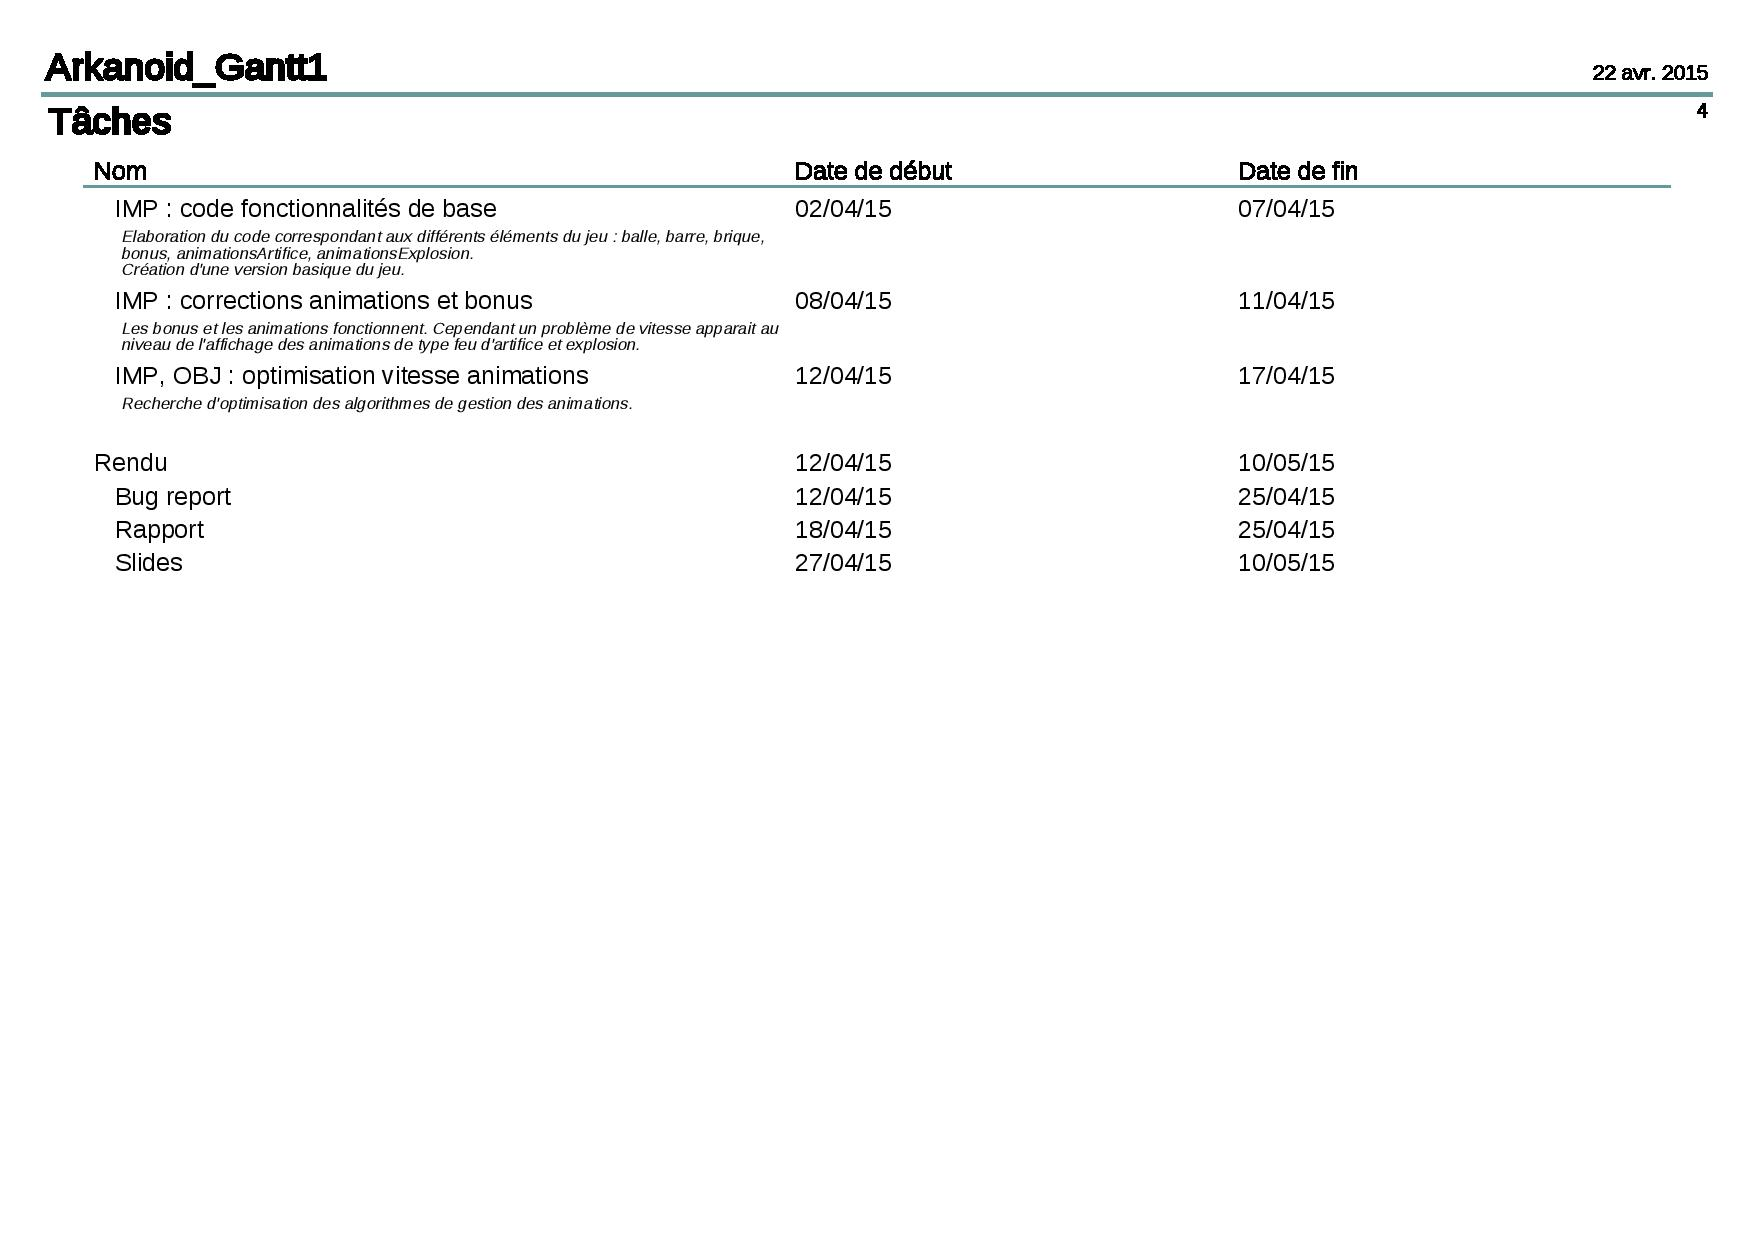
\includegraphics[width=1\textwidth]{img/WK3.jpg}\\
  \end{figure}
  
  \newpage
  \subsection{Diagramme de Gantt}
  	\begin{figure}[h!]
      \caption{Diagramme de Gantt}
      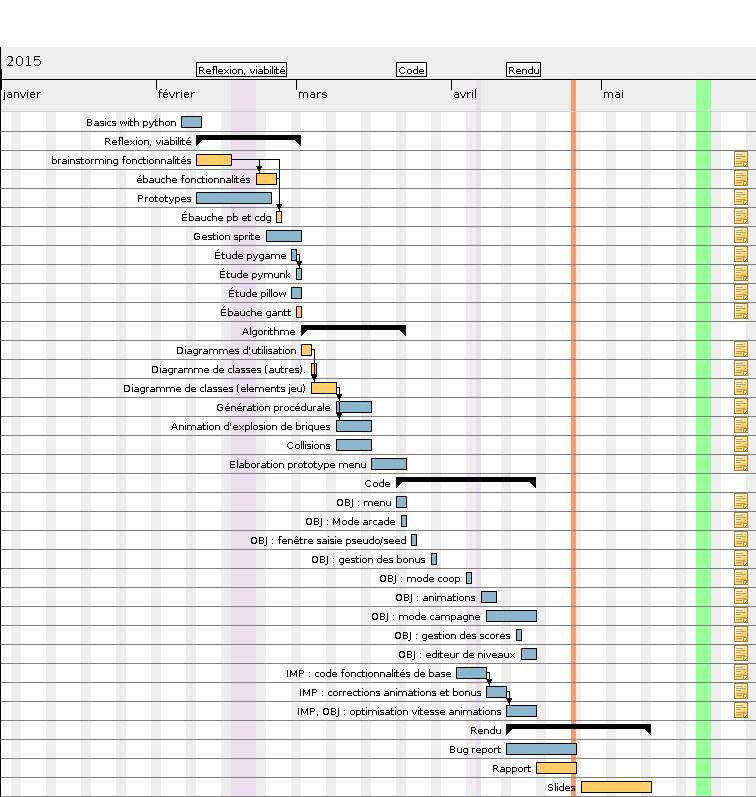
\includegraphics[width=1.1\textwidth]{img/gantt.jpg}\\[2em]
    \end{figure}
  
  \newpage
  \subsection{collision.py : fonction procgen}
  	\begin{minipage}{1\textwidth}
  	  \lstinputlisting[caption=fonction procgen, language=Python]{rsc/procgen.py}\nopagebreak
  	\end{minipage}
  	
  	Voir la section developpement technique pour de plus amples explications sur la stratégie adoptée. la fonction {\bf \em seed} (l 24), du module {\bf \em random}, permet de paramétrer la génération de nombre pseudo-aléatoire sur une graine. {\bf \em noise} correspond à une matrice de chiffre, correspondant aux pv des futurs briques. La fonction {\bf \em enlever} vient redéfinir certain de ces chiffres à 0. La variable {\em TESTING} n'est vrai que si et seulement si le programme est en test unitaire.

  \newpage
  \subsection{Working tree}
    \begin{figure}[hb!]
  	  \caption{Capture d'écran du working tree de git}
  	  \centering
  	  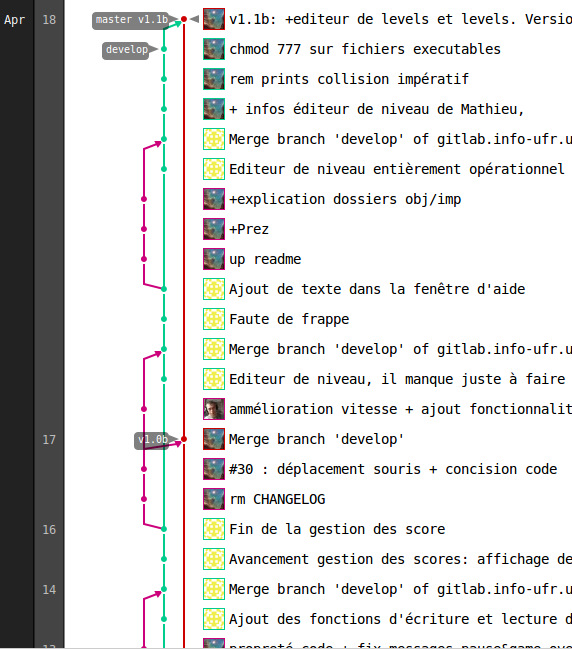
\includegraphics[width=1.1\textwidth]{img/workingtree.jpg}\\[2em]
  	\end{figure}
  	On pourra au passage noter notre gestion du système de tag
  
  \newpage
  \subsection{Issues}
  	\begin{figure}[hb!]
   	  \caption{Capture d'écran des issues de git}
  	  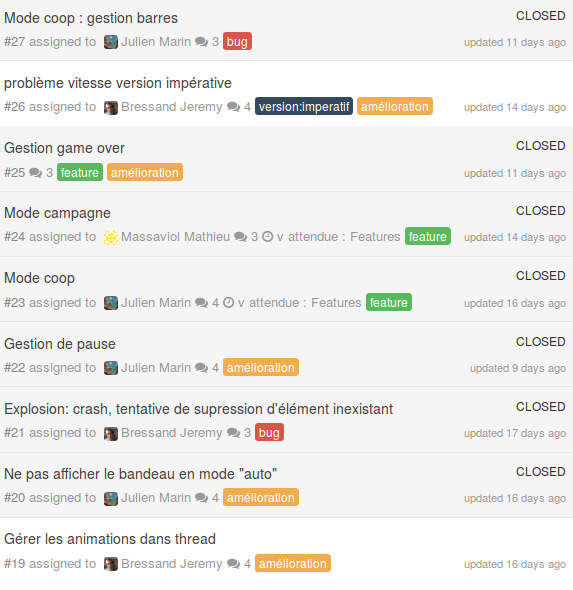
\includegraphics[width=1.1\textwidth]{img/issues.jpg}\\[2em]
  	\end{figure}
  
  \newpage
  \subsection{Bug report}
    \begin{enumerate}
       % Partie Jerem ...
       \item[\bf $\times$] Lorsque la balle est coincée entre la barre et le mur et que la barre fait pression contre la balle, la balle est éjectée de l'aire de jeu.

      \item[\checkmark] Bug variation vitesse balle lors de la collision avec la barre : Lors de la collision entre une balle et une barre, la vitesse de la balle varie de manière innatendue.
        \begin{itemize}
            \item[$\rightarrow$] Le problème a été résolu par un passage par angle, permettant d'obtenir une norme constante -- dans notre cas, une vitesse.
        \end{itemize}

      \item[\bf $\times$] Lorsque la barre reçoit le bonus d'agrandissement et qu'elle se trouve près du mur, elle se retrouve coincée dans celui ci.

      \item[\checkmark] Des briques supposées avoir un nombre de point de vie différents sont détruites au bout du même nombre de coups.
        \begin{itemize}
            \item[$\rightarrow$] Le problème était dû à une comparaison "inférieure" au lieu de "inférieure ou égale".
        \end{itemize}

      \item[\bf $\times$] Lors de collision balle/barre, il arrive dans de rares cas que la balle ne rebondisse pas de manière logique : elle inverse sa direction horizontale au lieu de sa direction verticale, ou inversement. 
       % Partie Marin
      \item[\checkmark] Crash du jeu lorsqu'une brique explosive en détruit plusieurs autres.
        \begin{itemize}
            \item[$\rightarrow$] Le programme éssayait de supprimer des briques déjà supprimées. Nous avons donc effectué la suppression avec la gestion de l'explosion.
        \end{itemize}
      \item[\checkmark] En mode coopératif, la position des barres des deux joueurs s'inversent, et une barre n'est pas supprimée - laissant une troisième barre "fantôme".
      \begin{itemize}
        \item[$\rightarrow$] Rien de conceptuel, nous avions simplement codé le mode coop trop rapidement.
      \end{itemize}

      \item[\checkmark] Vitesse anormale de la balle lorsqu'elle heurte un bord vertical d'une barre en mouvement.
      \begin{itemize}
        \item[$\rightarrow$] On ajoutait la vitesse de la barre à la balle, afin d'éviter qu'elles se retrouvent l'une dans l'autre. On a résolu le problème en plafonnant la vitesse horizontale de la balle à celle de la barre dans ce cas.
      \end{itemize}
      \item[\bf $\times$] Lorsque l'on commence une partie après en avoir finie une (ie être retourné au menu), le jeu commence en pause
      \item[\bf $\times$] En version imperative, le bonus d'ajout de balle créée une balle bien plus lente que les autres jusqu'à collision avec la barre.
    \end{enumerate}
  


\end{document}